\section{Theorie}
\label{sec:Theorie}

Ein Lock-In Verstärker wird häufig verwendet, um verrauschte Signale zu messen,
indem eine zu messende Signalspannung mit einer Referenzspannung einer bestimmten
Frequenz $\omega_0$ moduliert wird.
Er besteht im Wesentlichen aus einem Bandpass, einem Phasenschieber, einem Mischer
und einem Tiefpassfilter. Der schematische Aufbau eines Lock-In Verstärkers ist
in \ref{fig:schema} zu sehen.

\begin{figure}
  \centering
  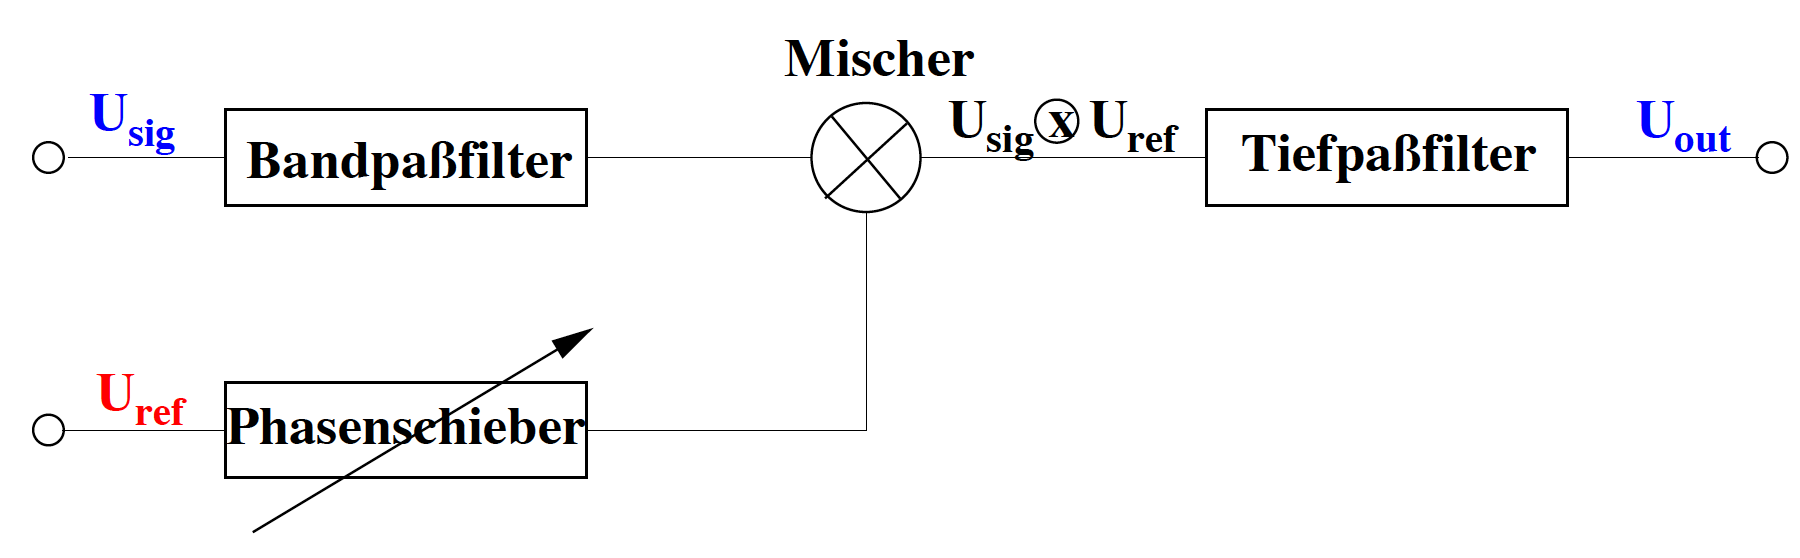
\includegraphics{data/schema.png}
  \caption{Schematische Darstellung der Funktionsweise eines Lock-In Verstärkers}
  \label{fig:schema}
\end{figure}


Im Folgenden soll die Funktionsweise eines Lock-In Verstärkers kurz erläutert
werden. Im Bandpass werden zunächst sehr hohe und sehr tiefe Frequenzen der
Signalspannung $U_{\symup{sig}}$ herausfiltert. In einem Mischer wird die
Signalspannung $U_{\symup{sig}}$ mit einer Referenzspannung $U_{\symup{ref}}$
multipliziert (gefaltet?!). Dabei hat die Referenzspannung eine feste Kreisfrequenz
$\omega_0$ und eine durch einen Phasenschieber anpassbare Phase $\phi$. Die Phase
ist dabei so zu wählen, dass die Referenzspannung $U_{\symup{ref}}$ mit der
Signalspannung $U_{\symup{sig}}$ synchron verläuft. Das gemischte Signal wird
daraufhin in einem Tiefpass über mehrer Perioden integriert. Dabei muss darauf
geachtet werden, dass  die Zeitkonstante $\tao=RC$ des Tiefpasses viel kleiner
ist, als die Frequenz der Spannung. Dabei werden alle Frequenzen, die nicht
der synchronisierten Referenzfrequenz entsprechen herausgefiltert und es entsteht
eine Ausgangsspannung $U_{\symup{out}}$, die Proportional zur Signalspannung
$U_{\symup{sig}}$ ist. Außerdem gilt der Zusammenhang
\begin{equation}
  U_{\symup{out}}\propto U_0 \cos(\phi) \,.
\end{equation}
